\chapter{Implémentation d'ENLSIP en Julia}\label{Implementation}

Ce chapitre a pour but de décrire la retranscription en Julia de l'algorithme ENLSIP que j'ai réalisée et dont les aspects théoriques ont été décrits au 
chapitre~\ref{Travail}. Nous discuterons également les choix faits en terme de programmation pour tirer parti au mieux des spécificités de Julia. Enfin, les 
résultats numériques obtenus sur les différents tests effectués seront présentés.

\section{Approche globale}

L'objectif est de produire un algorithme d'optimisation appliquant la méthode ENLSIP et obtenant les mêmes résultats, à la précision machine près,
que la version en Fortran77. C'est pour cette raison que j'ai mis en \oe uvre le même déroulement d'ensemble que celui présenté en~\eqref{algo:model enlsip}.
Sur conseil de mon maître de stage, j'ai repris la quasi-totalité des fonctions Fortran appelées dans l'algorithme afin de favoriser la concordance des deux implémentations.

Comme mon travail a pour finalité d'être déployé en contexte industriel par \HQ, les similarités entre les deux versions s'étendent aussi
à la nature des paramètres donnés en entrée pour exécuter le solveur. 

Un aspect sous-jacent de ce projet étant d'améliorer la maintenance de l'algorithme, j'ai également cherché à améliorer l'accessibilité de certaines portions du code,
jugées plus difficiles à appréhender en Fortran77.

Pour les fonctions où il a été difficile d'extraire les aspects théoriques, je n'ai pas cherché à complètement modifier le code. J'ai plutôt tâché de retranscrire le plus 
fidèlement possible ce qui était fait en Fortran77 en adaptant seulement la syntaxe au langage Julia.

\section{Utilisation de librairies Julia}

Bien qu'ENLSIP fasse appel à des fonctions issues de certaines libraires, notament LINPACK pour tout ce qui a trait aux calculs d'algèbre linéaire, le langage Julia donne accès
à un nombre important de librairies présentant des caractéristiques intéressantes.

\subsection*{Module LinearAlgebra}

Comme vu au chapitre~\ref{Travail}, le calcul matriciel, la factorisation QR et la résolution de systèmes linéaires occupent une place très importante dans la méthode ENLSIP.
On en retrouve notamment dans l'estimation des multiplicateurs de Lagrange ainsi que dans le calcul de la direction de descente.

Pour implémenter ces fonctionnalités, je me suis servi de la librairie Julia \texttt{LinearAlgebra}. Cette dernière comprend une grande quantité de fonctions pour le calcul matriciel
dont la plupart sont héritées de l'API OpenBLAS. Les aspects théoriques des fonctions disponibles sont majoritairement issus des travaux de~\citet{goluvanl13}. Cet ouvrage présente des méthodes de calcul matriciel
avantageuses en termes de complexité temporelle et spatiale.

L'exploitation de ce module a grandement contribué à améliorer la lisibilité du code. Par exemple la factorisation QR d'une matrice s'obtient par un appel à une seule
fonction. Il est également possible de faire pivoter les colonnes de la matrice de départ pour obtenir un résultat analogue à celui présenté en~\eqref{fact_qr}.
La version Fortran77 effectue, quant à elle, d'avantages d'étapes de calcul intermédiaires. 

De même, la résolution de systèmes linéaires triangulaires a bénéficié du passage à Julia. D'une part, cette opération ne nécessite qu'un seul appel de fonction;
d'autre part, Julia étant un langage fortement typé, la structure des matrices triangulaires est exploitée pour améliorer les performances de la résolution.



\subsection*{Module Polynomials}

Comme vu en~\ref{calcul_pas}, le calcul du pas fait intervenir des calculs de polynômes à minimiser sur un intervalle donné. Je me suis donc servi du module
\texttt{Polynomials} qui permet de modéliser des polynômes à partir de leurs coefficients. La méthode pour la longueur de pas ne faisant intervenir que des polynômes de degré 4,
j'ai également eu un accès facilité au calcul direct des racines et extrema.

Néanmoins, en comparant certains résultats intermédiaires d'ENLSIP-Fortran avec ceux de mon implémentation en Julia, j'ai constaté certaines différences qui amenaient à 
des longueurs de pas différentes. J'ai donc réduit l'utilisation de la librairie \texttt{Polynomials} et ai retranscrit certaines fonctions Fortran. Ainsi j'ai réussi 
à obtenir des résultats identiques.


\section{Gestion des variables internes}

Un autre aspect important concerne la gestion des variables internes dans le déroulement global du solveur d'un point de vue algorithmique.

Ayant été con\c cu à une période où les contraintes de mémoire des ordinateurs étaient fortes, la lisibilité du code Fortran77 d'ENLSIP s'en retrouve fortement 
touchée.
En effet, la plupart des variables de l'algorithme sont modifiées dans le corps même des différentes fonctions. Cela implique qu'une variable peut prendre différentes valeurs ayant 
une signification différente selon les fonctions où elle intervient.

Cette logique d'économie de la mémoire n'est plus vraiment d'actualité et ce indépendamment de l'utilisation du langage Julia. En revanche, dans le but de correspondre à l'algorithme en Fortran,
j'ai maintenu ce paradigme de modifier les variables dans le corps même des fonctions. Cela a nécessité certaines adaptations car en Julia il n'est par exemple pas possible de sauvegarder
les modifications de nombres entiers ou flottants. C'est néanmoins possible sur les objets s'apparentant à des structures de données, comme les \texttt{arrays}.

Puisque Julia offre la possibilité de créer ses propres types via l'utilisation de \texttt{structures}, j'ai pu adapter mon implémentation et mettre en place des éléments
absentes du codage d'ENLSIP en Fortran77. En effet, j'ai favorisé l'intégration de nouvelles structures de données, comportant différents attributs, pour une gestion plus efficace des variables de l'algorithme.

Les différents types que j'ai créés et implémentés sont listés ci-dessous:
\begin{description}
    \item[Iteration:] contient toutes les informations utiles d'une itération passée (point initial, direction de descente, longueur de pas...);
    \item[WorkingSet:] comprend les indices des contraintes actives;
    \item[ActiveConstraint:] contient l'évaluation des contraintes actives ainsi que leur matrice jacobienne.
\end{description}

Les \texttt{structures} présentent également l'avantage de sauvegarder les modifications d'attributs réalisées dans le c\oe ur des fonctions. 

\section{Difficultés rencontrées}

Le code source fourni avec la librairie ENLSIP étant très documenté, je disposais d'une très bonne base pour transposer la méthode en Julia. L'algorithme ayant été 
utilisé sans être modifié par \HQ\ pendant près de trente ans, sa robustesse n'était plus à prouver et je savais également à quels résultats je devais aboutir.
C'est pour cela que j'ai volontairement limité les évolutions dans mon travail d'implémentation, hormis celles décrites ci-dessus. 

En revanche, l'analyse du code source en vue de comprendre ce que faisait chacune des fonctions intermédiaires s'est révélée être une tâche plus longue et minutieuse
que ce qui était initialement prévu. De plus, ma connaissance du Fortran, surtout dans sa version 77, était très lacunaire au début du projet. J'ai donc dû m'ajuster 
à une syntaxe différente de ce à quoi j'étais habitué dans un algorithme très complexe et mettant en \oe uvre une méthode d'optimisation dont je ne connaissais
pas tous les aspects théoriques.

Tout ce travail a néanmoins mené à la retranscription complète de l'algorithme en Julia, ce qui constitue déjà une étape importante du projet.


\section{Résultats numériques}\label{implementation:resultats}

Pour vérifier la bonne mise en \oe uvre de l'algorithme en Julia, plusieurs tests sur des problèmes de moindres carrés non linéaires sous contraintes ont été réalisés.
Au moment de l'écriture de ce rapport, je ne dispose pas encore des ressources nécessaires pour exécuter l'algorithme sur des problèmes se rapportant au contexte 
industriel d'\HQ. Les tests se restreignent donc à la résolution de problèmes mathématiques en petite dimension, soit avec au plus cinq paramètres.

Cela permet néanmoins d'examiner les deux points suivants: d'une part comparer la concordance des résultats entre les versions Julia et Fortran77 et d'autre part, comparer les performances
de cette méthode d'optimisation avec d'autres solveurs de programmation non linéaire. 

La suite de cette section présente les résultats obtenus sur les différents tests qui ont pu être réalisés.

\subsection{\'Elaboration et modélisation des problèmes de test}

Les trois problèmes m'ayant servi de base de test sont extraits de la collection de problèmes d'optimisation de~\citet{hockschi}. Cet ouvrage comptabilise près 
d'une centaine de problèmes de programmation non linéaire sous contraintes con\c cus pour tester des algorithmes d'optimisation non linéaire. 

Chaque problème est documenté avec les informations suivantes:

\begin{itemize}
    \item l'expression analytique de la fonction objectif et des contraintes;
    \item un point initial;
    \item la solution attendue avec la valeur de la fonction objectif associée;
    \item les éventuelles données ou valeurs de paramètres nécessaires au calcul des contraintes ou de la fonction objectif.
\end{itemize}

Ces informations ont favorisé la vérification des résultats obtenus. Je n'ai volontairement pas fait de tests en modifiant le point départ. \'Etant donné que ma priorité 
était de vérifier que mon implémentation fonctionnait correctement, j'ai préféré me restreindre dans un cadre où les solutions et les points initiaux associés étaient connus.

Mon maître de stage et moi même avons sélectionné exclusivement des problèmes de moindres carrés, étant donné que c'est pour cette catégorie de problèmes que l'algorithme est
con\c cu. 

Les tests avec d'autres algorithmes d'optimisation se sont limités à l'utilisation de la version Julia du solveur open source IPOPT~\cite{andreas02}. Sa conception 
repose sur une méthode de points intérieurs avec une approche primal-dual.

Contrairement à ENLSIP, son emploi n'est pas restreint aux moindres carrés mais sa robustesse et sa capacité à résoudre des problèmes présentant des contraintes non linéaires 
en font un élément de comparaison pertinent. 



\subsection{Concordance avec ENLSIP-Fortran77}\label{compa_fortran}

Afin de comparer les résultats des deux implémentations d'ENLSIP, je me suis servi d'un problème test dont l'implémentation en Fortran77 avait déjà été proposée par~\citet{lindwedin88}.
Il s'agit du problème numéro 65 issu de~\cite{hockschi}; sa modélisation est donnée en~\eqref{pb65}:

\begin{equation}\label{pb65}
\left\{  
\begin{aligned}
&\min (x_1-x_2)^2 + \dfrac{(x_1+x_2-10)^2}{9}+(x_3-5)^2, \\ 
&\text{s.c.}\\
& 48-x_1^2-x_2^2-x_3^2 \geq 0,\\
&-4.5\leq x_i \leq 4.5,\text{ pour } i=1,2,\\
&-5 \leq x_3  \leq 5.
\end{aligned}  \right.
\end{equation}

\begin{description}
    \item[Point initial] $x_0 = (-5,5,0)^T$;
    \item[Solution attendue] $x^* = (3.650461821,3.65046168,4.6204170507)^T$;
    \item[Fonction objectif à la solution] $f(x^*) = 0.9535288567$.
\end{description}

La fonction objectif s'identifie à la norme au carré de la fonction de résidus:

\[ r : x\longmapsto  \left(x_1-x_2,\dfrac{x_1-x_2-10}{3},x_3-5\right)^T.\]


 Ce problème a également été une constante source d'améliorations de mon algorithme puisque j'ai pu l'utiliser en parallèle du développement de mon implémentation.
En effet, disposant des détails de chaque itération de l'exécution en Fortran77, j'ai pu apporter énormément de corrections à mon code en m'appuyant sur les différents résultats
intermédiaires observés en Fortran77 et que j'étais censé obtenir avec le code en Julia.

Les figures~\ref{fig:iter fortran} et~\ref{fig:iter julia} présentent le déroulement itération par itération des implémentations d'ENLSIP en Fortran et Julia. 
Les informations affichées correspondent aux grandeurs suivantes:

\begin{description}
    \item[(iter)] numéro de l'itération;
    \item[(fsum et objective)] valeur de la fonction objectif;
    \item[(hsum et cx\_sum)] norme du vecteur des contraintes actives; 
    \item[(dxnorm et $\|\text{p}\|$)] norme de la direction de descente; 
    \item[(koda, kocd et dimA, dimJ2)] dimensions utilisées pour le calcul de la direction de descente; 
    \item[(alpha et $\alpha$)] longueur de pas; 
    \item[(conv. speed)] facteur évaluant la vitesse de convergence; 
    \item[(max(w) et max weight)] la pénalité la plus élevée; 
    \item[(reduction)] diminution de la valeur de la fonction objectif; 
    \item[(working set)] indices des contraintes actives; 
\end{description}

\begin{figure}[ht]
    
    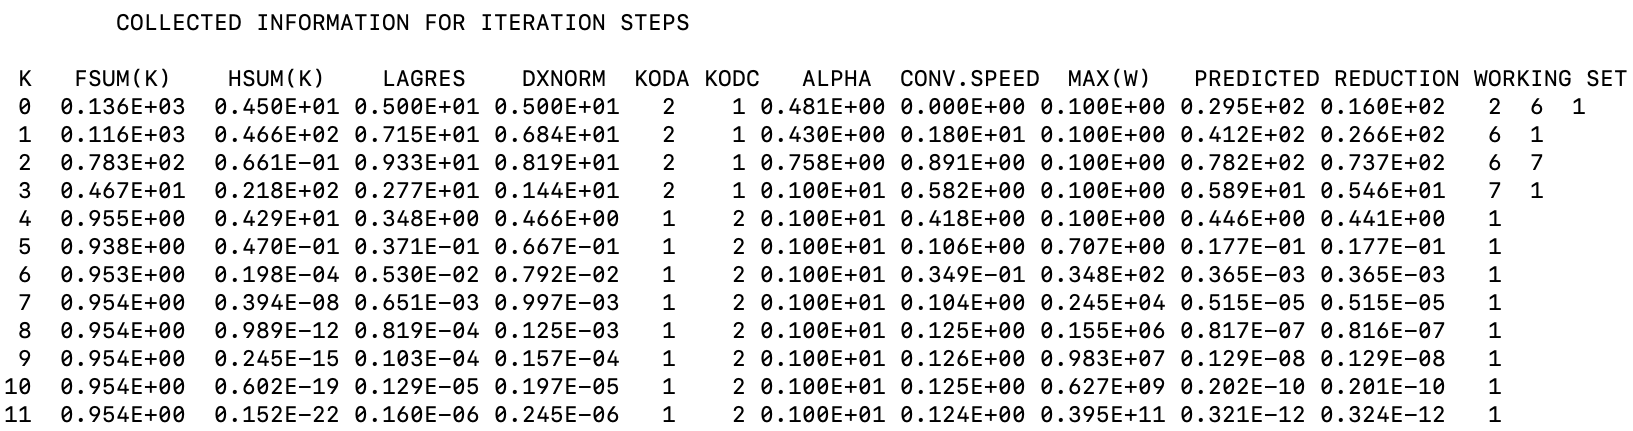
\includegraphics[scale=0.55]{FichiersSource/Images/sortie_f77_pb65}
    \caption{Itérations ENLSIP--Fortran sur le Pb65}
    \label{fig:iter fortran}
\end{figure}

\begin{figure}[ht]
    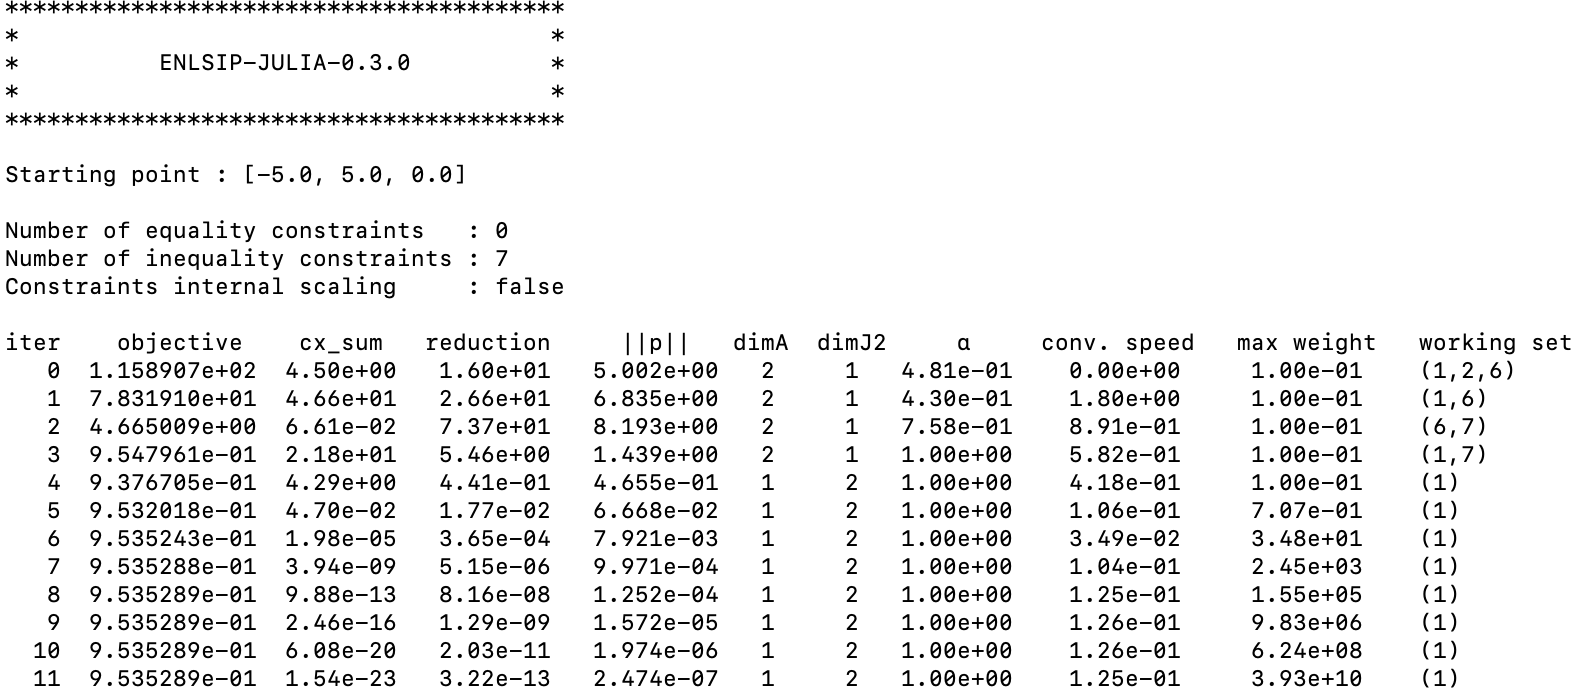
\includegraphics[scale=0.57]{FichiersSource/Images/sortie_pb65_julia}
    \caption{Itérations ENLSIP--Julia sur le Pb65}
    \label{fig:iter julia}
\end{figure}



On observe une concordance exacte des résultats intermédiaires obtenus et du nombre d'itérations effectuées. Cela prouve la bonne retranscription de 
la méthode, tout du moins sur ce problème. De futurs tests, réalisés à partir de modèles d'\HQ, permettront probablement de tirer de nouvelles conclusions à ce sujet.


\subsection{Comparaison des résultats et performances avec le solveur IPOPT}\label{compa_ipopt}

En plus du problème 65 déjà présenté, deux autres problèmes, le 57 et le 42 de la collection de~\citet{hockschi}, ont été utilisés afin de comparer les performances d'ENLSIP en Julia avec IPOPT.
Leurs modélisations et informations sont données respectivement en~\eqref{pb57} et en~\eqref{pb42}.

Commençons par la description du problème 57:

\begin{equation}\label{pb57}
 \left\{  
\begin{aligned} 
&\min f(x)= \sum\limits_{i=1}^{44} f_i(x)^2,\\ 
&\text{s.c.}\\
&0.49x_2-x_1x_2-0.09 \geq 0,\\
&x_1\geq 0.4,\  x_2 \geq -4.
\end{aligned} \right. 
\end{equation}

\begin{description}
    \item[Point initial] $x_0 = (0.42,5)^T$;
    \item[Solution attendue] $x^* = (0.419952675,1.284845629)^T$;
    \item[Fonction objectif à la solution] $f(x^*) =0.02845966972$,
\end{description}

avec $f_i(x) = b_i - x_1 - (0.49-x_1)\exp(-x_2(a_i-8)) \text{ pour }i=1,\ldots,44$. 

Les fonctions $f_i$ peuvent s'interpréter comme la différence entre l'observation $b_i$ et la prédiction du modèle de paramètres $x_1$ et $x_2$ réalisée en $a_i$.
Bien que cela reste un problème théorique, sa forme est bien adaptée au cas d'utilisation chez \HQ de l'algorithme ENLSIP. On peut s'attendre à une convergence vers la solution en un nombre plus faible 
d'itérations qu'avec IPOPT.

Les valeurs des données sont fournies dans l'ouvrage~\cite{hockschi}.

On remarque que le point initial est relativement proche de la solution attendue, en particulier la première composante. Ce problème s'est donc avéré être également un bon moyen de tester la robustesse de mon implémentation.

Passons désormais à la description du problème 42:

\begin{equation}
    \label{pb42}
\left\{  
\begin{aligned} 
&\min\ f(x)=(x_1-1)^2+(x_2-2)^2+(x_3-3)^2+(x_4-4)^2, \\ 
&\text{s.c.}\\
&x_1-2 = 0,\\
&x_3^2+x_4^2-2= 0.
\end{aligned} \right.
\end{equation}

\begin{description}
    \item[Point initial] $x_0 = (1,1,1,1)^T$;
    \item[Solution attendue] $x^* = (2,2,0.6\sqrt 2, 0.8\sqrt 2)^T$;
    \item[Fonction objectif à la solution] $f(x^*) =28-10\sqrt 2\approx 13.8578643$.
\end{description}

Le problème 42 peut sembler plus simple que les deux autres. Par exemple, la première contrainte impose directement la valeur du paramètre à l'optimum $x_1$.
Il présente néanmoins l'intérêt de n'avoir que des contraintes d'égalité et de partir d'un point non réalisable, ce qui permet d'éprouver la capacité de l'algorithme
à gérer ce genre de configurations.

Les différents tests ayant amené aux résultats présentés dans les tableaux~\ref{resultats:pb57},~\ref{resultats:pb42} et~\ref{resultats:pb65} ont été réalisés sur un ordinateur équipé d'un 
processeur IntelCore i5 de 10ème génération. La version $1.6.0$ de Julia a été utilisée et les temps de calcul ont été mesurés à l'aide de la librairie Julia \texttt{BenchmarkTools}. 

Le temps d'exécution n'a néanmoins pas pu être évalué sur ENLSIP-Fortran77.

\begin{table}
    \centering
    \begin{tabular}{|l|c|c|c|}
        \hline
        Solveur & Itérations & Temps de calcul &  Objectif \\ \hline
        ENLSIP-Julia & $5$ & $1.663\sec$ & $2.845966972\text{e-}02$ \\\hline
        IPOPT & $24$ & $2.003\sec$ & $2.845966907\text{e-}02$\\ \hline
    \end{tabular}  
    \caption{Comparaison d'ENLSIP-Julia avec IPOPT sur le problème 57}
    \label{resultats:pb57}
\end{table}

\begin{table}
    \centering
    \begin{tabular}{|l|c|c|c|}
        \hline
        Solveur & Itérations & Temps de calcul &  Objectif \\ \hline
        ENLSIP-Julia & $15$ & $1.493\sec$ & $1.385786438\text{e+}01$ \\\hline
        IPOPT & $10$ & $1.584\sec$ & $1.385786437\text{e+}01$\\ \hline
    \end{tabular}  
    \caption{Comparaison d'ENLSIP-Julia et IPOPT sur le problème 42}
    \label{resultats:pb42}
\end{table}

\begin{table}
    \centering
    \begin{tabular}{|l|c|c|c|}
        \hline
        Solveur & Itérations & Temps de calcul &  Objectif \\ \hline
        ENLSIP-Fortran77 & $11$ & -- & $0.953529\text{e+}01$ \\\hline
        ENLSIP-Julia & $11$ & $1.585\sec$ & $0.953528856\text{e+}01$\\\hline
        IPOPT & $12$ & $2.372\sec$ & $0.953528856\text{e+}01$\\ \hline
    \end{tabular}  
    \caption{Comparaison d'ENLSIP avec IPOPT sur le problème 65}
    \label{resultats:pb65}
\end{table}


Plusieurs constats peuvent être tirés de ces résultats. Tout d'abord, les minima trouvés par les deux algorithmes sont extrêmement proches, voire quasiment identiques, 
les différences apparaissant à partir de la huitième ou neuvième décimale selon les problèmes. L'objectif de parvenir à trouver des résultats corrects avec l'implémentation en Julia
d'ENLSIP semble donc globalement atteint.

En termes de performances, les temps de calcul d'ENLSIP-Julia remplissent largement les exigences fixées au chapitre~\ref{Besoins} et sont du même ordre de grandeur
que ceux d'IPOPT. Ce dernier point s'explique sûrement par le fait que les problèmes testés sont de très petite dimension et ne permettent donc pas de tirer des conclusions sur les différences 
de vitesse d'exécution. 

Ces premiers résultats se révèlent donc très encourageants pour la suite du développement d'ENLSIP en Julia.
Comme dit précédemment, d'autres tests seront réalisés sur des problèmes en plus grande dimension afin de se rapprocher petit à petit des problèmes effectivement résolus par l'outil 
de prévision dont \HQ\ se sert en production.